Test D

Die Wahl des Zahlungsmodells ist von entscheidender Bedeutung, um den besten Preis für die vertraglich vereinbarten Dienstleistungen zu erzielen.

Die drei von Amazon Web Services angebotenen Zahlungsmodelle werden im Folgenden dargestellt.
\\\\
Die On-Demand-Option erfordert keine langfristigen Verpflichtungen, sie ist daher die teuerste Alternative, die auf Stundenbasis berechnet wird. Die Saving Plans erfordern den Abschluss von Verträgen über 1 oder 3 Jahre, um günstige Preise zu erhalten.
\\Spots schließlich sind die billigste Option, haben aber den Nachteil, dass ihre Verfügbarkeit nicht immer garantiert ist.
\\\\
Jedes Zahlungsmodell hat ihre Vor- und Nachteile und eignet sich für unterschiedliche Anwendungsfälle. Gute Ergebnisse können auch durch die Kombination mehrerer Zahlungsmodelle erzielt werden.
\\\\
( noch in Arbeit =>)
Vor- und Nachteile noch tabellarisch aufzulisten!!
%https://youtu.be/Q5wSvUVPyYY?t=678

%On-Demand
%Commitment options
%Excess capacity/Spot Instances

\subsection{On-Demand / Nutzungsabhängige Zahlung}
Bei diesem Zahlungsmodell besteht keine Notwendigkeit, Budgets festzulegen. Die Kosten richten sich nach dem Verbrauch auf der Grundlage der Nutzungsstunden.
\\
Dieses Modell eignet sich für Projekte, bei denen nicht viel vorhersehbar ist und die Möglichkeit besteht, dass das Projekt in kurzer Zeit abgeschlossen sein wird, so dass es keinen Sinn macht, eine langfristige Verpflichtung einzugehen.
\\
Hier einige Beispiele von EC2-Instanzen in On-Demand Zahlungsmodell.

\begin{center}
      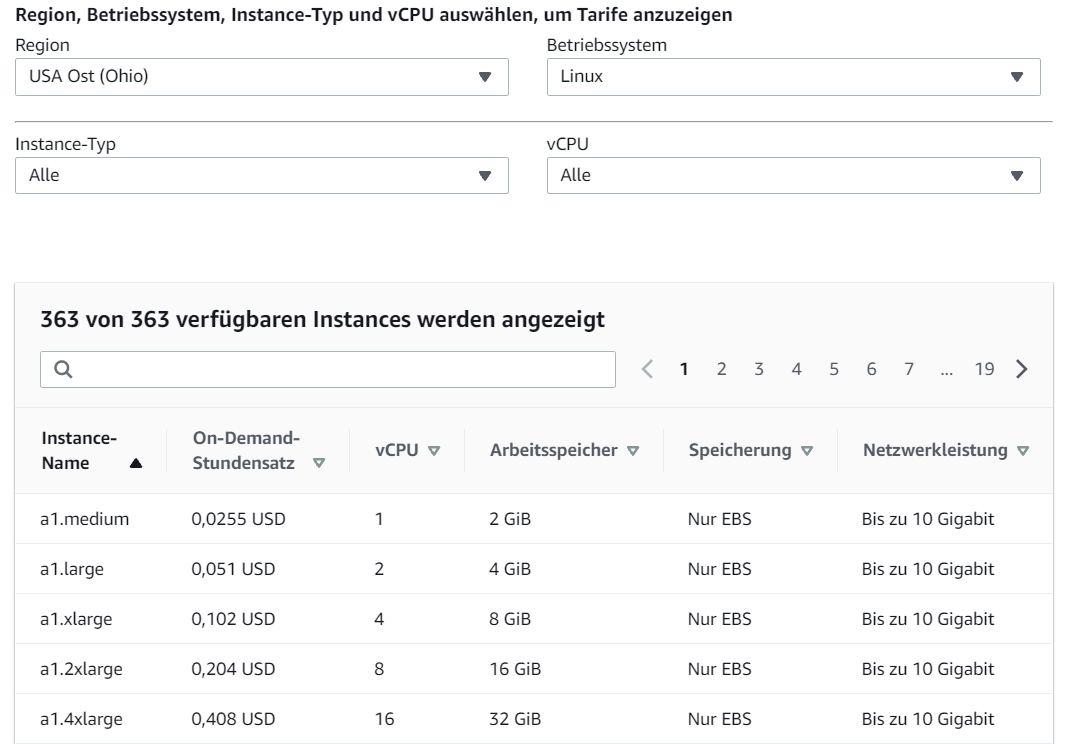
\includegraphics[scale=0.4]{sources/On-Demand-Pläne für Amazon EC2}\label{fig:OnDemand_Preise}\\
      \textbf{Abbildung \autoref{fig:OnDemand_Preise}:} On-Demand Preise für Amazon EC2
      {\cite{AMZ01}}
\end{center}
\subsection{Reservierte Instanzen und Saving Plans}
%https://www.youtube.com/watch?v=c_zlPQimrvY
\begin{flushleft}
Diese beiden Zahlungsmodelle sind sich sehr ähnlich. Beide kommen mit einer Nutzungsverpflichtung, die in \$-€/Stunden gemessen wird.

Um die reduzierten Preise bekommen zu können, müssen Verträge 1 oder 3 Jahre abgeschlossen werden.

Nachfolgend werden die prozentualen Einsparungen gemäß dem jeweiligen Modell gezeigt.
\end{flushleft}

\begin{table}[h!]
    \centering
\begin{tabular}{ |p{3cm}||p{3cm}|p{3.6cm}|p{3.6cm}|  }
    \hline
    \multicolumn{4}{|c|}{Einsparungen nach Modell}                                                   \\
    \hline
    Compute Savings Plans & EC2-Instance-Savings-Plans & Convertible Reserved Instances & Standard Reserved Instances \\
    \hline
    66\%& 72\%
    & 1 J. (31 \%), 3 J. (54\%)  & 1 J. (40 \%), 3 J.(60\%)
    \\
    \hline
\end{tabular}
\end{table}

Folgenden Attributen definieren den Preis von RI:
AUCH FÜR SAVING PLANS?
\\
.
\\
-
\\
-
\\

%\\
EC2 Spot-Instances können mit On-Demand, Reserved Instances und Saving-Plans kombiniert werden, um sowohl feste als auch dynamische Last abzudecken.

    %3 Arten von S. Plans: Compute and EC2 Instance
    {\cite{AMZ07}}

\subsection{Versteigerung? / Spot Instanzen }
EC2 Spot-Instances bieten die Möglichkeit aus ungenutzter EC2-Instances zu profitieren.
Mit einem Preisvorteil von bis zu 90 \% gegenüber normalen On-Demand-Instanzen sind Spot-Instanzen ideal für fehlertolerante Anwendungen wie auf Containern ausgeführte Workloads, CI/CD, Bigdata-Anwendungen und ähnliches.
%unterbrechbar
%https://aws.amazon.com/de/ec2/spot/pricing/
\subsection{Wann welches Zahlungsmodell?}
(To-Do:) Was sind die Kriterien für die Auswahl eines oder mehrerer Zahlungsmodelle?
%MACH EINE SCHÖNE GRAFIK
%https://youtu.be/mKEdhmJ2udA?t=79


%Automate the selection to get the best price
%https://spot.io/aws-cost-optimization-calculator/

\subsection{Vorauszahlung}
Zusätzlich zu den oben beschriebenen Zahlungsmodellen motivieren uns einige Anbieter von Cloud-Diensten, im Voraus zu zahlen, im Austausch bieten sie bessere Preise. Dies ist bei Amazon der Fall, das derzeit (2021) drei verschiedene Optionen anbietet: keine, teilweise und vollständige Vorauszahlung.

Bei teilweiser Vorauszahlung ist eine Anzahlung von etwa 50\% zu leisten.

(To-Do: wie viel kann in den verschiedenen Szenarien eingespart werden).